\chapter[Anteproyecto]{Anteproyecto} \label{sec:anteproyecto}

% -----------------------------------------------------------------------------------------------%
\section{Introducción}
Los CubeSat son un tipo de satélites en miniatura desarrollados en módulos de 10x10x10 cm (1U). Año a año, estos nanosatélites adquieren más relevancia debido a su relativamente bajo costo de desarrollo y lanzamiento. Actualmente, miles de estos satélites operan en órbita terrestre baja (LEO, Low Earth Orbit) desempeñando diversas funciones en misiones científicas, tecnológicas y de telecomunicaciones.

El proyecto tiene como objetivo el desarrollo de un amplificador de potencia (PA, Power Amplifier) diseñado para operar en la Banda S de frecuencia, orientado a una futura integración en satélites CubeSat. 

Dado que se trata de una aplicación de potencia en el espacio, el diseño se enfoca fuertemente en alcanzar una alta eficiencia energética. La alta eficiencia no solo permite un mejor aprovechamiento de la energía, recurso sumamente escaso en el espacio, sino que también minimiza la generación de calor, fundamental en este tipo de aplicaciones debido a la dificultosa tarea de disiparlo.

Además de la eficiencia energética, otros desafíos tecnológicos clave deben ser abordados en el trabajo. Entre estos se encuentran la miniaturización del módulo, reducción de costos de desarrollo y fabricación, y lograr inmunidad ante fenómenos adversos como la radiación o temperatura.

Dentro de este contexto, dónde soluciones altamente eficientes son muy demandadas, el diseño de un PA de gran eficiencia resulta crítico para optimizar los recursos limitados como la energía y el espacio. Bajo esta premisa, el presente trabajo busca satisfacer las necesidades mencionadas.

% -----------------------------------------------------------------------------------------------%
\subsection{Motivación}
La motivación del trabajo surge del interés de los integrantes del grupo de poder llevar a cabo proyectos de potencia en radiofrecuencia (RF) que provean soluciones a problemas reales de la coyuntura actual. Esta motivación unió sus fuerzas con el deseo del grupo GiAR, perteneciente a la Universidad Tecnológica Nacional de Buenos Aires, de lanzar un satélite CubeSat al espacio.

% -----------------------------------------------------------------------------------------------%
\subsection{Método}
Para llevar a cabo el proyecto se diseñará un amplificador de topología Doherty. Este se compone por un acoplador híbrido en cuadratura (etapa desfasadora), un amplificador de operación permanente (carrier amplifier) y uno de cresta (peaking amplifier), como ilustra el diagrama en bloques de la Fig.~\ref{fig:doherty_blocks}. Esta topología provee una eficiencia considerable y buena linealidad, lo cual posibilita el empleo de señales con modulación de amplitud (QAM, por ejemplo), muy utilizadas en aplicaciones espaciales. 

\begin{figure}[H]
    \centering
    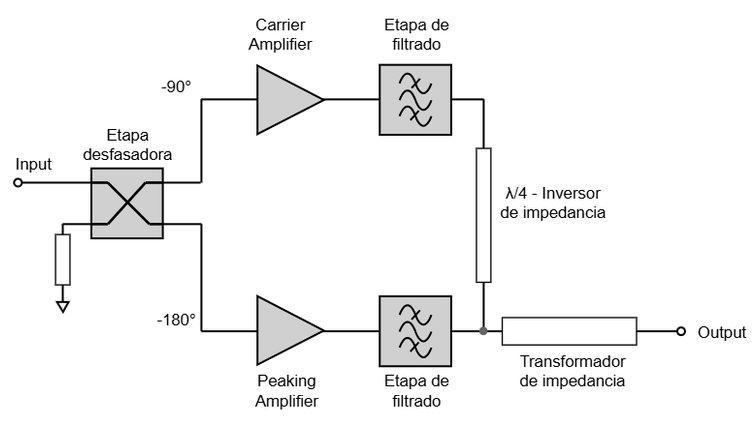
\includegraphics[width=0.7\linewidth]{Figures/doherty.png}
    \caption{Diagrama en bloques de la topología Doherty.}
    \label{fig:doherty_blocks} 
\end{figure}

Los transistores a utilizar para el diseño de los amplificadores son de tecnología GaN. La razón de esta elección es su buen manejo de potencia y linealidad. 

Para diseño, simulación e implementación del PA se utilizarán herramientas como Altium Designer y ANSYS. 
La gestión del proyecto será llevada a cabo empleando la metodología Kanban, empleando Trello, con el objetivo de optimizar y agilizar el flujo de trabajo con el planteo de hitos realizables en el corto plazo.

% -----------------------------------------------------------------------------------------------%
\section{Tema de Investigación}
Como se ha mencionado previamente, en los últimos años los costos asociados al desarrollo y lanzamiento de satélites se han reducido considerablemente gracias al auge de plataformas como los CubeSat. Sin embargo, estos valores continúan siendo significativos. Por esta razón, es indispensable contar con un conocimiento profundo de las posibles fallas y fenómenos adversos que podrían afectar a los sistemas que componen al satélite una vez en órbita. Minimizar estos riesgos es esencial para evitar que una misión fracase y el satélite quede reducido a basura espacial. 

Entre las variables más críticas a considerar en el diseño de sistemas electrónicos para el espacio se encuentra la temperatura. En órbita terrestre baja, los CubeSat se ven expuestos a variaciones térmicas extremas, provocadas principalmente por los ciclos de exposición directa al sol. A esto se suma el hecho de que, en el espacio, no existe la posibilidad de disipar el calor por convección, lo que limita de forma significativa la capacidad de disipación.

En el presente trabajo, el sistema a desarrollar es un amplificador de potencia, el cual constantemente disipa una fracción de la energía que consume en forma de calor. Si no se gestionan adecuadamente estas pérdidas, se corre el riesgo de sobrecalentamiento, lo cual puede provocar desvíos en los parámetros del amplificador e incluso daños permanentes en el dispositivo.

Otra variable fundamental en el entorno espacial es la radiación. Los dispositivos electrónicos a bordo están expuestos a partículas de alta energía, como protones y electrones, además de rayos cósmicos. Esta exposición puede generar efectos acumulativos (TID, Total Ionizing Dose) o eventos puntuales (SEEs, Single Event Effects) que alteren el comportamiento eléctrico de los circuitos. En el caso particular de un PA, se busca estudiar si estos fenómenos podrían inducir variaciones en parámetros críticos como la ganancia, impedancia, eficiencia o punto de compresión.

Frente a estas problemáticas, se plantea como tema de investigación el diseño, desarrollo y caracterización de un amplificador de potencia de alta eficiencia energética, destinado a aplicaciones espaciales, con énfasis en su evaluación ante condiciones adversas. Para ello, el dispositivo será sometido a ensayos que simulen las condiciones reales a las que se enfrentaría en una misión, con el fin de identificar las posibles degradaciones en su rendimiento y establecer criterios de diseño que aseguren su estabilidad y confiabilidad.

Este enfoque permitirá generar conocimientos valiosos en torno al comportamiento de dispositivos de potencia en el espacio y sentar las bases para futuros desarrollos robustos, eficientes y adaptados a las exigencias del entorno. Así, se apunta a contribuir con soluciones tecnológicas viables para plataformas satelitales emergentes, en línea con las crecientes demandas del sector aeroespacial.

\section{Gestión del Alcance}
Para poder llevar a cabo una gestión efectiva del alcance del proyecto se plantearon los objetivos de la Tabla 1. Estos se hallan divididos en cuatro categorías que remarcan su criticidad (a la vez que su factibilidad) dentro del contexto del proyecto. Los objetivos indicados como mandatorios son los que el proyecto debe cumplir obligatoriamente y se considera factible realizar. Los deseables también son considerados como factibles pero no son absolutamente críticos para el éxito del proyecto. Los opcionales son aquellos que harán del proyecto, en caso de cumplirse, un diseño más atractivo pero no están ligados al objetivo principal de este trabajo. Por último, se encuentran los objetivos no incluidos en el proyecto actual.

\begin{table}[H]
    \centering
    \caption{Clasificación de requisitos de diseño del amplificador.}
    \label{tab:requisitos_clasificados}
    \renewcommand{\arraystretch}{1.1}
    \begin{tabular}{cccc}
        \hline\hline
        \textbf{Mandatorios} & \textbf{Deseables} & \textbf{Opcionales} & \textbf{No incluidos} \\
        \hline
        $f_{c} = 2{,}2$ GHz  & OIP3 $\ge 35$ dBm  & Tolerancia a rad.   & ---        \\
        $BW = 35$ MHz        & $BW = 10 \%$       & ---                 & Modulación \\
        $P_{out} \ge 1$ W    & $P_{out} \ge 2$ W  & ---                 & ---        \\
        PAE $\ge 35 \%$      & PAE $\ge 50 \%$    & ---                 & ---        \\
        \hline\hline
    \end{tabular}
\end{table}

\subsection{Hitos}
Una vez definidos los objetivos del proyecto, se establecieron los hitos a partir de los cuales se organiza el trabajo a llevar a cabo. Cada hito representa un fragmento de todo el proyecto y da como resultado, de ser completado satisfactoriamente, un entregable. En la Tabla \ref{tab:mapa_hitos} se muestra cada uno de ellos, junto con su descripción y entregable correspondiente.

\begin{xltabular}{\textwidth}{>{\centering\arraybackslash}p{0.6cm} X X p{2.5cm}}
    \caption{Mapa de hitos del proyecto del amplificador de potencia.} \label{tab:mapa_hitos} \\
    \hline
    \textbf{\#} & \textbf{Hito} & \textbf{Descripción} & \textbf{Entregable} \\
    \hline
    \endfirsthead

    \multicolumn{4}{c}{\textit{Continuación del Cuadro~\ref{tab:mapa_hitos}}} \\
    \hline
    \textbf{\#} & \textbf{Hito} & \textbf{Descripción} & \textbf{Entregable} \\
    \hline
    \endhead

    \hline
    \endfoot

    \hline
    \endlastfoot

    1 & Diseño y simulación clase B y acoplador en ADS & Diseño y simulación en ADS de un amplificador clase B y acoplador. & Archivos de simulación \\
    
    \hline
    2 & Diseño de PCB clase B y acoplador & Incluye revisiones internas. Incluye tener definida la BOM teniendo en cuenta la fabricación en JLCPCB. & Archivos gerber \\
    
    \hline
    3 & Pedido del diseño clase B y acoplador & Realizar el pedido en China. Incluye cargar gerber en JLCPCB, elegir las especificaciones, incluye el sourcing de las partes. & Comprobante de pedido \\
    
    \hline
    4 & Diseño y simulación clase C & Diseño y simulación en ADS de un amplificador clase C. & Archivos de simulación \\
    
    \hline
    5 & Diseño PCB clase C & Incluye revisiones internas. Incluye tener definida la BOM teniendo en cuenta la fabricación en JLCPCB. & Archivos gerber \\
    
    \hline
    6 & PCBs Clase B y acoplador en mano & El día 9 de junio deben haber llegado los PCBs enviados a fabricar y ensamblar en JLCPCB. & PCBs \\
    
    \hline
    7 & Medición y caracterización de los PCBs & Se realizan todas las mediciones necesarias a los PCBs fabricados. & Resultados de medición \\
    
    \hline
    8 & Primera irradiación & Se realizará la irradiación del amplificador clase B y del acoplador. & Foto irradiando \\
    
    \hline
    \rowcolor[HTML]{b6d7a8} \multicolumn{4}{c}{\textbf{Parciales y finales (30/06 a 19/07)}} \\
    
    \hline
    9 & Diseño pasivos Doherty y presentación de resultados de la radiación & Se diseñarán el resto de componentes pasivos de la topología Doherty en ADS. Además se presentarán los resultados de la radiación. & Archivos de simulación y resultados de medición \\
    
    \hline
    10 & Integración del diseño de los pasivos con el amplificador de \textit{peaking} en ADS & Diseño en ADS para integrar los pasivos al amplificador clase C. & Archivos de simulación \\
    
    \hline
    11 & Diseño de PCB del amplificador de \textit{peaking} con sus pasivos & Se realizará el PCB en Altium incluyendo los pasivos en el diseño logrado anteriormente. & Archivos gerber \\
    
    \hline
    12 & Pedido del diseño clase C y red de salida & Realizar el pedido en China. Incluye cargar gerber en JLCPCB, elegir las especificaciones, incluye el \textit{sourcing} de las partes. & Comprobante de pedido \\
    
    \hline
    13 & Simulación en ADS del PCB final, completamente integrado & Diseño en ADS del amplificador Doherty. & Archivos de simulación \\
    
    \hline
    14 & Fabricación de los PCBs de \textit{peaking} y pasivos Doherty & El día X deben haber llegado los PCBs enviados a fabricar y ensamblar en JLCPCB. & PCBs \\
    
    \hline
    15 & Medición y caracterización de los PCBs & Se realizan todas las mediciones necesarias a los PCBs fabricados (en condiciones de realizar pruebas sobre el diseño final). & Resultados de medición \\
    
    \hline
    16 & ADS - Ajuste del diseño del PCB final, completamente integrado & Se ajustan los valores del diseño final en función de las mediciones del amplificador clase C. & Archivos de simulación \\
    
    \hline
    17 & Diseño PCB Doherty & PCB del diseño final. & Archivos gerber \\
    
    \hline
    18 & Pedido del diseño final & Pedido del diseño final en China. & Comprobante de envío \\
    
    \hline
    19 & Tener el PCB del diseño final en mano & Tener el PCB del diseño final en mano habiendo llegado de China. & PCBs \\
    
    \hline
    20 & Medición y caracterización del PCB final & Se realizan todas las mediciones necesarias a los PCBs fabricados del diseño final. & Resultados de medición \\
    
    \hline
    \rowcolor[HTML]{b6d7a8} \multicolumn{4}{c}{\textbf{Baja actividad - Parciales y finales (03/11 a 05/12)}} \\
    
    \hline
    21 & Irradiación del diseño final & Irradiar el diseño final. Probablemente con menor disponibilidad debido a parciales. & Foto irradiando \\
    
    \hline
    22 & Presentación de los resultados de la irradiación & Se presentarán los resultados de la irradiación. & Resultados de medición \\
    
    \hline
    \rowcolor[HTML]{b6d7a8} \multicolumn{4}{c}{\textbf{Fin de diseño y medición}} \\
    
    \hline
    23 & Paper - Trabajo de investigación & Se espera para esta fecha tener la versión final del paper escrita para la publicación definitiva. & Paper \\

    \hline
\end{xltabular}

\subsection{Desglose de Tareas}
Si bien cada hito sirve como un pantallazo general del progreso del proyecto, es imperativo desglosar cada uno de ellos en tareas (y a su vez estas en subtareas) para lograr una división precisa y efectiva del trabajo entre los integrantes del equipo de trabajo. A continuación se muestran las tablas de desglose de tareas para cada hito presentado.

% hito 1
\begin{table}[H]
    \centering
    \renewcommand{\arraystretch}{1.1}
    \begin{tabularx}{\textwidth}{|C{1cm}|C{1.6cm}|Y|Y|}
        \hline
        \multicolumn{4}{|l|}{\textbf{Hito 1 - Diseño Amplificador clase B y acoplador}} \\
        \hline
        \textbf{\#} & \textbf{Subtarea} & \textbf{Título} & \textbf{Descripción} \\ \hline
        1.1 & & Simulación en ADS           & \\ \hline
        1.2 & & Optimización del diseño     & \\ \hline
        1.3 & & Diseño final + simulaciones & \\ \hline
        1.4 & & Revisión interna            & \\
        \hline
    \end{tabularx}
\end{table}

% hito 2
\begin{table}[H]
    \centering
    \renewcommand{\arraystretch}{1.1}
    \begin{tabularx}{\textwidth}{|C{1cm}|C{1.6cm}|Y|Y|}
        \hline
        \multicolumn{4}{|l|}{\textbf{Hito 2 - Diseño de PCB - Clase B y acoplador}} \\
        \hline
        \textbf{\#} & \textbf{Subtarea} & \textbf{Título} & \textbf{Descripción} \\ \hline
        2.1 & & Exportar diseño acoplador            & \\ \hline
        2.2 & & Diseño PCB acoplador                 & \\ \hline
        2.3 & & Esquemático + BOM clase B            & \\ \hline
        2.4 & & Dibujo líneas de transmisión clase B & \\ \hline
        2.5 & & Diseño PCB clase B                   & \\ \hline
        2.6 & & Revisión interna                     & \\
        \hline
    \end{tabularx}
\end{table}

% hito 3
\begin{table}[H]
    \centering
    \renewcommand{\arraystretch}{1.1}
    \begin{tabularx}{\textwidth}{|C{1cm}|C{1.6cm}|Y|Y|}
        \hline
        \multicolumn{4}{|l|}{\textbf{Hito 3 - Pedido del diseño - Clase B y acoplador}} \\
        \hline
        \textbf{\#} & \textbf{Subtarea} & \textbf{Título} & \textbf{Descripción} \\ \hline
        3.1 & & Exportar archivos de fabricación             & \\ \hline
        3.2 & & Definir fabricante y sourcing de componentes & \\ \hline
        3.3 & & Realizar pedido                              & \\
        \hline
    \end{tabularx}
\end{table}

% hito 4
\begin{table}[H]
    \centering
    \renewcommand{\arraystretch}{1.1}
    \begin{tabularx}{\textwidth}{|C{1cm}|C{1.6cm}|Y|Y|}
        \hline
        \multicolumn{4}{|l|}{\textbf{Hito 4 - Diseño y Simulación - Clase C}} \\
        \hline
        \textbf{\#} & \textbf{Subtarea} & \textbf{Título} & \textbf{Descripción} \\ \hline
        4.1 &       & Marco teórico clase C            & \\ \hline
        4.2 &       & Diseño en ADS                    & \\ \cline{2-4}
            & 4.2.1 & Armado del circuito ideal        & Polarización y circuito ideal \\ \cline{2-4}
            & 4.2.2 & Load-pull                        & \\ \cline{2-4}
            & 4.2.3 & Diseño redes de adaptación       & \\ \cline{2-4}
            & 4.2.4 & Optimización redes de adaptación & \\ \cline{2-4}
            & 4.2.5 & Búsqueda de componentes reales   & \\ \cline{2-4}
            & 4.2.6 & Diseño circuito real             & \\ \cline{2-4}
            & 4.2.7 & Optimización circuito real       & \\ \cline{2-4}
            & 4.2.8 & Análisis paramétrico + Robustez  & \\ \hline
        4.3 &       & Revisión interna                 & \\
        \hline
    \end{tabularx}
\end{table}

% hito 5
\begin{table}[H]
    \centering
    \renewcommand{\arraystretch}{1.1}
    \begin{tabularx}{\textwidth}{|C{1cm}|C{1.6cm}|Y|Y|}
        \hline
        \multicolumn{4}{|l|}{\textbf{Hito 5 - Diseño PCB - Clase C}} \\
        \hline
        \textbf{\#} & \textbf{Subtarea} & \textbf{Título} & \textbf{Descripción} \\ \hline
        5.1 &        & Diseño esquemático                  & \\ \cline{2-4}
            & 5.1.1  & Dibujo del circuito simulado en ADS & \\ \cline{2-4}
            & 5.1.2  & Asignación de footprints            & \\ \hline
        5.2 &        & Armado BOM & Excel con part numbers de todos los componentes \\ \hline
        5.3 &        & Diseño PCB                          & \\ \cline{2-4}
            & 5.3.1  & Placement de componentes & Definición boardshape y placement \\ \cline{2-4}
            & 5.3.2  & Dibujo líneas de transmisión        & \\ \cline{2-4}
            & 5.3.3  & Completar PCB                       & \\ \hline
        5.4 &        & Revisión interna                    & \\
        \hline
    \end{tabularx}
\end{table}

% hito 6
\begin{table}[H]
    \centering
    \renewcommand{\arraystretch}{1.1}
    \begin{tabularx}{\textwidth}{|C{1cm}|C{1.6cm}|Y|Y|}
        \hline
        \multicolumn{4}{|l|}{\textbf{Hito 6 - Tener los PCBs Clase B y acoplador en mano}} \\
        \hline
        \textbf{\#} & \textbf{Subtarea} & \textbf{Título} & \textbf{Descripción} \\ \hline
        6.1 & & Llevar y retirar los PCBs en Outsource para ensamblaje & \\
        \hline
    \end{tabularx}
\end{table}

% hito 7
\begin{table}[H]
    \centering
    \renewcommand{\arraystretch}{1.1}
    \begin{tabularx}{\textwidth}{|C{1cm}|C{1.6cm}|Y|Y|}
        \hline
        \multicolumn{4}{|l|}{\textbf{Hito 7 - Medición y caracterización de los PCBs}} \\
        \hline
        \textbf{\#} & \textbf{Subtarea} & \textbf{Título} & \textbf{Descripción} \\ \hline
        7.1 & 7.1.1 & Coordinación fecha grupo & \\ \cline{2-4}
            & 7.1.2 & Coordinación con tutor   & Hablar con un tutor para que nos asista con las mediciones (Carlos Navarro, Manuel García, Alejandro Henze, Matías Hampel) \\ \hline
        7.2 &       & Reserva del laboratorio y equipos & \\ \hline
        7.3 &       & Planeamiento del experimento      & \\ \hline
        7.4 &       & Mediciones                        & \\ \hline
        7.5 &       & Informe interno & Análisis de resultados y presentación informe interno \\
        \hline
    \end{tabularx}
\end{table}

% hito 8
\begin{table}[H]
    \centering
    \renewcommand{\arraystretch}{1.1}
    \begin{tabularx}{\textwidth}{|C{1cm}|C{1.6cm}|Y|Y|}
        \hline
        \multicolumn{4}{|l|}{\textbf{Hito 8 - Primera Irradiación}} \\
        \hline
        \textbf{\#} & \textbf{Subtarea} & \textbf{Título} & \textbf{Descripción} \\ \hline
        8.1 & & Marco teórico irradiación        & \\ \hline
        8.2 & & Definir experimento a realizar   & \\ \hline
        8.3 & & Pedido de turno                  & \\ \hline
        8.4 & & Preparar instrumental necesario  & Solicitar instrumental en caso de ser necesario \\ \hline
        8.5 & & Medición                         & \\
        \hline
    \end{tabularx}
\end{table}

% hito 9
\begin{table}[H]
    \centering
    \renewcommand{\arraystretch}{1.1}
    \begin{tabularx}{\textwidth}{|C{1cm}|C{1.6cm}|Y|Y|}
        \hline
        \multicolumn{4}{|l|}{\textbf{Hito 9 - Diseño Pasivos Doherty y Resultados de Radiación}} \\
        \hline
        \textbf{\#} & \textbf{Subtarea} & \textbf{Título} & \textbf{Descripción} \\ \hline
        9.1 &       & Análisis de resultados                   & Informe explicando lo que se obtuvo del experimento \\ \hline
        9.2 &       & Diseño de pasivos en ADS                 & \\ \hline
            & 9.2.1 & Armado de circuito ideal                 & \\ \hline
            & 9.2.2 & Simulación y análisis del circuito ideal & \\ \hline
            & 9.2.3 & Armado de circuito real                  & \\ \hline
            & 9.2.4 & Simulación y análisis del circuito real  & \\ \hline
            & 9.2.5 & Optimización                             & \\ \hline
            & 9.2.6 & Simulación EM                            & \\ \hline
        9.3 &       & Revisión interna                         & \\ \hline
        9.4 &       & Simulación EM con ANSYS o CST            & \\
        \hline
    \end{tabularx}
\end{table}

% hito 10
\begin{table}[H]
    \centering
    \renewcommand{\arraystretch}{1.1}
    \begin{tabularx}{\textwidth}{|C{1cm}|C{1.6cm}|Y|Y|}
        \hline
        \multicolumn{4}{|l|}{\textbf{Hito 10 - Integración del diseño de pasivos con clase C en ADS}} \\
        \hline
        \textbf{\#} & \textbf{Subtarea} & \textbf{Título} & \textbf{Descripción} \\ \hline
        10.1 & & Simulación pasivos + clase C & \\ \hline
        10.2 & & Optimización                 & \\ \hline
        10.3 & & Revisión interna             & \\
        \hline
    \end{tabularx}
\end{table}

% hito 11
\begin{table}[H]
    \centering
    \renewcommand{\arraystretch}{1.1}
    \begin{tabularx}{\textwidth}{|C{1cm}|C{1.6cm}|Y|Y|}
        \hline
        \multicolumn{4}{|l|}{\textbf{Hito 11 - Diseño PCB amplificador clase C con pasivos}} \\
        \hline
        \textbf{\#} & \textbf{Subtarea} & \textbf{Título} & \textbf{Descripción} \\ \hline
        11.1 &         & Diseño esquemático                  & \\ \cline{2-4}
             & 11.1.1  & Dibujo del circuito simulado en ADS & \\ \cline{2-4}
             & 11.1.2  & Asignación de footprints            & \\ \hline
        11.2 &         & Armado BOM & Excel con part numbers de todos los componentes \\ \hline
        11.3 &         & Diseño PCB                          & \\ \cline{2-4}
             & 11.3.1  & Placement de componentes            & \\ \cline{2-4}
             & 11.3.2  & Dibujo líneas de transmisión        & \\ \cline{2-4}
             & 11.3.3  & Completar PCB                       & \\ \hline
        11.4 &         & Revisión interna                    & \\
        \hline
    \end{tabularx}
\end{table}

% hito 12
\begin{table}[H]
    \centering
    \renewcommand{\arraystretch}{1.1}
    \begin{tabularx}{\textwidth}{|C{1cm}|C{1.6cm}|Y|Y|}
        \hline
        \multicolumn{4}{|l|}{\textbf{Hito 12 - Pedido del diseño clase C y pasivos}} \\
        \hline
        \textbf{\#} & \textbf{Subtarea} & \textbf{Título} & \textbf{Descripción} \\ \hline
        12.1 & & Exportar archivos de fabricación             & Gerber y drill \\ \hline
        12.2 & & Definir fabricante y sourcing de componentes & \\ \hline
        12.3 & & Realizar pedido                              & \\
        \hline
    \end{tabularx}
\end{table}

% hito 13
\begin{table}[H]
    \centering
    \renewcommand{\arraystretch}{1.1}
    \begin{tabularx}{\textwidth}{|C{1cm}|C{1.6cm}|Y|Y|}
        \hline
        \multicolumn{4}{|l|}{\textbf{Hito 13 - Simulación en ADS del PCB final}} \\
        \hline
        \textbf{\#} & \textbf{Subtarea} & \textbf{Título} & \textbf{Descripción} \\ \hline
        13.1 &         & Pensar el diseño                  & \\ \hline
        13.2 &         & Diseño en ADS                     & \\ \cline{2-4}
             & 13.2.1  & Armado circuito ideal             & Polarización y circuito ideal \\ \cline{2-4}
             & 13.2.2  & Optimización redes de adaptación  & \\ \cline{2-4}
             & 13.2.3  & Búsqueda de componentes reales    & \\ \cline{2-4}
             & 13.2.4  & Diseño circuito real              & \\ \cline{2-4}
             & 13.2.5  & Optimización circuito real        & \\ \cline{2-4}
             & 13.2.6  & Análisis paramétrico + robustez   & \\ \hline
        13.3 &         & Revisión interna                  & \\
        \hline
    \end{tabularx}
\end{table}

% hito 14
\begin{table}[H]
    \centering
    \renewcommand{\arraystretch}{1.1}
    \begin{tabularx}{\textwidth}{|C{1cm}|C{1.6cm}|Y|Y|}
        \hline
        \multicolumn{4}{|l|}{\textbf{Hito 14 - Fabricación de los PCBs peaking y pasivos Doherty}} \\
        \hline
        \textbf{\#} & \textbf{Subtarea} & \textbf{Título} & \textbf{Descripción} \\ \hline
        14.1 & & Llevar y retirar los PCBs en Outsource para ensamblaje & \\
        \hline
    \end{tabularx}
\end{table}

% hito 15
\begin{table}[H]
    \centering
    \renewcommand{\arraystretch}{1.1}
    \begin{tabularx}{\textwidth}{|C{1cm}|C{1.6cm}|Y|Y|}
        \hline
        \multicolumn{4}{|l|}{\textbf{Hito 15 - Medición y caracterización de los PCBs}} \\
        \hline
        \textbf{\#} & \textbf{Subtarea} & \textbf{Título} & \textbf{Descripción} \\ \hline
        15.1 & 15.1.1 & Coordinación fecha           & \\ \cline{2-4}
             & 15.1.2 & Coordinación con tutor       & \\ \hline
        15.2 &        & Reserva del laboratorio y equipos & \\ \hline
        15.3 &        & Planeamiento del experimento      & \\ \hline
        15.4 &        & Mediciones                        & \\ \hline
        15.5 &        & Informe interno & Análisis de resultados y presentación informe interno \\
        \hline
    \end{tabularx}
\end{table}

% hito 16
\begin{table}[H]
    \centering
    \renewcommand{\arraystretch}{1.1}
    \begin{tabularx}{\textwidth}{|C{1cm}|C{1.6cm}|Y|Y|}
        \hline
        \multicolumn{4}{|l|}{\textbf{Hito 16 - ADS. Ajuste del diseño del PCB final}} \\
        \hline
        \textbf{\#} & \textbf{Subtarea} & \textbf{Título} & \textbf{Descripción} \\ \hline
        16.1 & 16.1.1 & Análisis del circuito real a partir de valores obtenidos en el clase C & \\ \cline{2-4}
             & 16.1.2 & Optimización del circuito real  & \\ \cline{2-4}
             & 16.1.3 & Análisis paramétrico + robustez & \\ \hline
        16.2 &        & Revisión interna                & \\
        \hline
    \end{tabularx}
\end{table}

% hito 17
\begin{table}[H]
    \centering
    \renewcommand{\arraystretch}{1.1}
    \begin{tabularx}{\textwidth}{|C{1cm}|C{1.6cm}|Y|Y|}
        \hline
        \multicolumn{4}{|l|}{\textbf{Hito 17 - Diseño PCB Doherty}} \\
        \hline
        \textbf{\#} & \textbf{Subtarea} & \textbf{Título} & \textbf{Descripción} \\ \hline
        17.1 &         & Diseño esquemático                  & \\ \cline{2-4}
             & 17.1.1  & Dibujo del circuito simulado en ADS & \\ \cline{2-4}
             & 17.1.2  & Asignación de footprints            & \\ \hline
        17.2 &         & Armado BOM                          & \\ \hline
        17.3 &         & Diseño PCB                          & \\ \cline{2-4}
             & 17.3.1  & Placement de componentes            & \\ \cline{2-4}
             & 17.3.2  & Dibujo líneas de transmisión        & \\ \cline{2-4}
             & 17.3.3  & Completar PCB                       & \\ \hline
        17.4 &         & Revisión interna                    & \\
        \hline
    \end{tabularx}
\end{table}

% hito 18
\begin{table}[H]
    \centering
    \renewcommand{\arraystretch}{1.1}
    \begin{tabularx}{\textwidth}{|C{1cm}|C{1.6cm}|Y|Y|}
        \hline
        \multicolumn{4}{|l|}{\textbf{Hito 18 - Pedido del diseño final}} \\
        \hline
        \textbf{\#} & \textbf{Subtarea} & \textbf{Título} & \textbf{Descripción} \\ \hline
        18.1 & & Exportar archivos de fabricación             & Gerber y drill \\ \hline
        18.2 & & Definir fabricante y sourcing de componentes & \\ \hline
        18.3 & & Realizar pedido                              & \\
        \hline
    \end{tabularx}
\end{table}

% hito 19
\begin{table}[H]
    \centering
    \renewcommand{\arraystretch}{1.1}
    \begin{tabularx}{\textwidth}{|C{1cm}|C{1.6cm}|Y|Y|}
        \hline
        \multicolumn{4}{|l|}{\textbf{Hito 19 - PCB final en mano}} \\
        \hline
        \textbf{\#} & \textbf{Subtarea} & \textbf{Título} & \textbf{Descripción} \\ \hline
        19.1 & & Llevar y retirar los PCBs en Outsource para ensamblaje & \\
        \hline
    \end{tabularx}
\end{table}

% hito 20
\begin{table}[H]
    \centering
    \renewcommand{\arraystretch}{1.1}
    \begin{tabularx}{\textwidth}{|C{1cm}|C{1.6cm}|Y|Y|}
        \hline
        \multicolumn{4}{|l|}{\textbf{Hito 20 - Medición y caracterización PCB final}} \\
        \hline
        \textbf{\#} & \textbf{Subtarea} & \textbf{Título} & \textbf{Descripción} \\ \hline
        20.1 & 20.1.1 & Coordinación fecha grupo & \\ \cline{2-4}
             & 20.1.2 & Coordinación con tutor   & Hablar con un tutor para que nos asista con las mediciones (Carlos Navarro, Manuel García, Alejandro Henze, Matías Hampel) \\ \hline
        20.2 &        & Reserva del laboratorio y equipos & \\ \hline
        20.3 &        & Planeamiento del experimento      & \\ \hline
        20.4 &        & Mediciones                        & \\ \hline
        20.5 &        & Informe interno & Análisis de resultados y presentación informe interno \\
        \hline
    \end{tabularx}
\end{table}

% hito 21
\begin{table}[H]
    \centering
    \renewcommand{\arraystretch}{1.1}
    \begin{tabularx}{\textwidth}{|C{1cm}|C{1.6cm}|Y|Y|}
        \hline
        \multicolumn{4}{|l|}{\textbf{Hito 21 - Irradiación del diseño final}} \\
        \hline
        \textbf{\#} & \textbf{Subtarea} & \textbf{Título} & \textbf{Descripción} \\ \hline
        21.1 & & Marco teórico irradiación      & \\ \hline
        21.2 & & Definir experimento a realizar & \\ \hline
        21.3 & & Pedido de turno                & \\ \hline
        21.4 & & Preparar instrumental          & Solicitar instrumental en caso de ser necesario \\ \hline
        21.5 & & Medición                       & \\
        \hline
    \end{tabularx}
\end{table}

% hito 22
\begin{table}[H]
    \centering
    \renewcommand{\arraystretch}{1.1}
    \begin{tabularx}{\textwidth}{|C{1cm}|C{1.6cm}|Y|Y|}
        \hline
        \multicolumn{4}{|l|}{\textbf{Hito 22 - Presentación resultados de irradiación}} \\
        \hline
        \textbf{\#} & \textbf{Subtarea} & \textbf{Título} & \textbf{Descripción} \\ \hline
        22.1 & & Análisis de resultados & Informe explicando lo obtenido del experimento \\
        \hline
    \end{tabularx}
\end{table}

% hito 23
\begin{table}[H]
    \centering
    \renewcommand{\arraystretch}{1.1}
    \begin{tabularx}{\textwidth}{|C{1cm}|C{1.6cm}|Y|Y|}
        \hline
        \multicolumn{4}{|l|}{\textbf{Hito 23 - Paper}} \\
        \hline
        \textbf{\#} & \textbf{Subtarea} & \textbf{Título} & \textbf{Descripción} \\ \hline
        23.1 & & Preparación marco teórico          & Búsqueda de referencias y papers \\ \hline
        23.2 & & Pensar qué decir y cómo            & \\ \hline
        23.3 & & Armar el esqueleto del paper       & \\ \hline
        23.4 & & Escribir el abstract               & \\ \hline
        23.5 & & Escribir las secciones             & \\ \hline
        23.6 & & Revisión por parte de otros grupos & \\ \hline
        23.7 & & Revisión por tutores docentes      & \\ \hline
        23.8 & & Publicación                        & \\
        \hline
    \end{tabularx}
\end{table}

\section{Gestión del Tiempo}
Un diagrama Gantt fue realizado para gestionar el tiempo del proyecto. Mediante el uso de este diagrama es posible determinar la factibilidad del desarrollo del proyecto dentro del tiempo establecido y, simultáneamente, identificar cuellos de botella, tareas que sea posible (o no) paralelizar y gestionar de mejor manera el tiempo de cada tarea.

El proyecto consta de varias etapas, algunas superpuestas temporalmente con otras. Tanto las etapas como su paralelización, en caso de haber, se ilustran en la Figura 2.

\section{Gestión del Riesgo}
La realización de una matriz de riesgos resultó importante para tener una visualización de todos los riesgos existentes a la vez que una ponderación de la relevancia de los mismos. 

Para hacer esto, a cada riesgo considerado se le asignó una probabilidad de ocurrencia y una magnitud al impacto del evento sobre el proyecto. En base a estos dos indicadores, se otorga al evento una calificación, la cual indica que tan importante es el atacar ese problema.

La probabilidad de ocurrencia se mide de 0 a 1, mientras que la magnitud podrá ser muy bajo, bajo, medio, alto y muy alto. A mayor probabilidad de ocurrencia y mayor magnitud de impacto mayor es la calificación que se le otorga al evento. Dicha calificación podrá ser bajo, medio, alto y muy alto. A continuación, la tabla con los eventos.

\small
\renewcommand{\arraystretch}{1.15}

\newcommand{\bajo}{\cellcolor{yellow!20}BAJO}
\newcommand{\medio}{\cellcolor{orange!25}MEDIO}
\newcommand{\alto}{\cellcolor{red!20}ALTO}
\newcommand{\muyalto}{\cellcolor{red!45}\textbf{MUY ALTO}}

\begin{xltabular}{\textwidth}{|>{\centering\arraybackslash}p{0.7cm}|p{4.0cm}|p{1.3cm}|p{1.2cm}|>{\centering\arraybackslash}p{0.8cm}|p{1.2cm}|}

\caption{Matriz de riesgos del proyecto.} \label{tab:risk_matrix} \\

\hline
\textbf{EDT} & \textbf{Descripción del evento de riesgo} & \textbf{Fuente} & \textbf{Imp.} & \textbf{Prob.} & \textbf{Calif.} \\
\hline
\endfirsthead

\multicolumn{4}{c}{\textit{Continuación del Cuadro~\ref{tab:mapa_hitos}}} \\
\hline
\textbf{EDT} & \textbf{Descripción del evento de riesgo} & \textbf{Fuente} & \textbf{Imp.} & \textbf{Prob.} & \textbf{Calif.} \\
\hline
\endhead

\hline
\endfoot

\hline
\endlastfoot

\multirow{2}{*}{3.2} & El sourcing de componentes se encuentra en un lugar diferente al ensamblaje. Pueden producirse tiempos y costos extras. & Logística & Medio & 0.7 & \alto \\ \cline{2-6}
& Es posible que Outsource no esté disponible. & Logística & Medio & 0.5 & \medio \\ \hline
3.3 & Costos extras de aduana. & Econ. & Muy bajo & 0.8 & \bajo \\ \hline

4.2.1 & No se puede realizar un buen análisis de estabilidad y el circuito puede volverse inestable. & Técnico & Alto & 0.2 & \medio \\ \hline
4.2.5 & No existan componentes adecuados. & Tecnol. & Bajo & 0.2 & \bajo \\ \hline
4.2.8 & Que resulte un circuito poco robusto. & Técnico & Medio & 0.25 & \bajo \\ \hline

5.1.2 & Error en la asignación de algún footprint. & Operativo & Alto & 0.2 & \medio \\ \hline

6.1 & Es posible que Outsource no esté disponible. & Logística & Medio & 0.5 & \medio \\ \hline

\multirow{2}{*}{7.4} & Mediciones que no dan bien. & Técnico & Alto & 0.3 & \alto \\ \cline{2-6}
& Destrucción del dispositivo por alta potencia manejada. & Técnico & Muy Alto & 0.1 & \medio \\ \hline

\multirow{2}{*}{8.3} & Demora en la asignación de turno. & Operativo & Bajo & 0.4 & \bajo \\ \cline{2-6}
& Indisponibilidad del experimento. & Operativo & Alto & 0.1 & \bajo \\ \hline
8.4 & Indisponibilidad del instrumental. & Operativo & Alto & 0.2 & \medio \\ \hline

9.1 & Obtención de resultados no significativos. & Técnico & Medio & 0.5 & \medio \\ \hline

10.1 & Integración fallida. Se deberá rediseñar. & Técnico & Medio & 0.25 & \bajo \\ \hline

11.1.2 & Error en la asignación de algún footprint. & Operativo & Alto & 0.1 & \bajo \\ \hline

\multirow{2}{*}{12.2} & El sourcing de componentes se encuentra en un lugar diferente al ensamblaje. Pueden producirse tiempos y costos extras. & Logística & Medio & 0.7 & \alto \\ \cline{2-6}
& Es posible que Outsource no esté disponible. & Logística & Medio & 0.5 & \medio \\ \hline
12.3 & Costos extras de aduana. & Econ. & Muy bajo & 0.8 & \bajo \\ \hline

13.2.4 & Imposibilidad de integrar el diseño de un amplificador Doherty. & Técnico & Medio & 0.5 & \bajo \\ \hline
13.2.6 & Que resulte un circuito poco robusto. & Técnico & Medio & 0.25 & \bajo \\ \hline

14.1 & Es posible que Outsource no esté disponible. & Logística & Medio & 0.5 & \medio \\ \hline

15.4 & Mediciones que no dan bien. & Técnico & Alto & 0.3 & \medio \\ \hline

16.2.3 & Diseño final poco robusto. & Técnico & Medio & 0.5 & \medio \\ \hline

\multirow{2}{*}{18.2} & El sourcing de componentes se encuentra en un lugar diferente al ensamblaje. Pueden producirse tiempos y costos extras. & Logística & Bajo & 0.7 & \medio \\ \cline{2-6}
& Es posible que Outsource no esté disponible. & Logística & Bajo & 0.5 & \bajo \\ \hline
18.3 & Costos extras de aduana. & Econ. & Muy bajo & 0.8 & \bajo \\ \hline

19.1 & Es posible que Outsource no esté disponible. & Logística & Bajo & 0.6 & \bajo \\ \hline

20.4 & Mediciones que no dan bien en el diseño final. & Técnico & Bajo & 0.5 & \bajo \\ \hline

21.2 & Es posible que el PCB final exceda el tamaño máximo del experimento. & Operativo & Medio & 0.5 & \medio \\ \hline
21.4 & Indisponibilidad del instrumental. & Operativo & Medio & 0.25 & \bajo \\ \hline

22.1 & Obtención de resultados no significativos. & Técnico & Alto & 0.75 & \muyalto \\ \hline

23.8 & Paper rechazado. & Tecnol. & Muy Alto & 0.5 & \alto \\ \hline

\end{xltabular}

El análisis de las estrategias a tomar ante los riesgos fue realizado una vez que se habían enviado a ensamblar las placas del amplificador de carrier y donde nos disponíamos a realizar las mediciones, es decir en el hito número 7. Es por eso que se plantearon estrategias a partir de este punto. 
Las estrategias se enfocan en los eventos de impacto medio y alto en el proyecto, ya que son éstos los que tendrán un efecto mayor en el éxito del proyecto.

Por último, cabe destacar que luego de realizado el presente análisis de riesgo, se midió la placa del amplificador de carrier, la cual dio dentro de los valores esperados. Éste amplificador cumple con los objetivos mínimos del proyecto, lo que tiene como consecuencia una reducción generalizada del riesgo del proyecto.

\section{Gestión de Calidad}
En pos de poder visualizar rápidamente el cumplimiento de tiempos y objetivos del proyecto, resulta pertinente emplear un método para la gestión de calidad del mismo. Se implementará un sistema de indicadores los cuales revelarán, de manera cuantitativa, el estado de cada una de las partes claves del proyecto. Los indicadores se dividen en dos categorías: por un lado, aquellos asociados a parámetros del hardware desarrollado, por el otro, los relacionados a la planificación y gestión del proyecto.

En pos de poder visualizar rápidamente el cumplimiento de tiempos y objetivos del proyecto, resulta pertinente emplear un método para la gestión de calidad del mismo. Se implementará un sistema de indicadores los cuales revelarán, de manera cuantitativa, el estado de cada una de las partes claves del proyecto. Los indicadores se dividen en dos categorías: por un lado, aquellos asociados a parámetros del hardware desarrollado, por el otro, los relacionados a la planificación y gestión del proyecto.

\textbf{Indicadores de Hardware}
\begin{itemize}
    \item \textbf{Máxima potencia de salida.} Fuente: ensayos de laboratorio Indica la potencia máxima que el amplificador puede entregar sin comprometer la integridad del PCB ni degradar otros parámetros del amplificador.
    \item \textbf{Ganancia del amplificador.} Fuente: ensayos de laboratorio. Indica el cociente entre potencia de salida y potencia inyectada a la entrada.
    \item \textbf{Eficiencia del amplificador.} Fuente: ensayos de laboratorio. Cociente entre la potencia de salida y la potencia total consumida para obtener esa señal de salida.
    \item \textbf{Desviación de la frecuencia central.} Fuente: ensayos de laboratorio. Indica, de manera porcentual, el corrimiento de la frecuencia central real respecto de la prevista (2,2 GHz).
    \item \textbf{Linealidad (o distorsión) de la señal de salida.} Fuente: ensayos de laboratorio. Evalúa la fidelidad de la señal amplificada, útil para determinar la viabilidad de uso de modulaciones de ciertas modulaciones complejas (QAM). Se medirá a través de parámetros como el punto de intercepción de tercer orden (OIP3) y la distorsión armónica total (THD).
    \item \textbf{Área ocupada por el PCB.} Fuente: diseño CAD. Siendo la placa parte de un CubeSat, cuyo espacio es limitado, se evaluará el área total ocupada por el PCB.
\end{itemize}

\textbf{Indicadores del Proyecto}
\begin{itemize}
    \item \textbf{Retraso respecto del Gantt.} Medido como la diferencia entre tareas efectivamente completadas y tareas planificadas para una determinada fecha.
    \item \textbf{Porcentaje de entregables cumplidos.} Indica cuántos entregables han sido completados satisfactoriamente en relación al total. Refleja el grado de avance del proyecto.
    \item \textbf{Cantidad de iteraciones de diseño.} Indica la cantidad de ciclos de diseño, prueba y ajuste que fueron necesarios para alcanzar los objetivos y parámetros deseados. Da una representación de la eficiencia del proceso de diseño.
\end{itemize}

